\documentclass[10pt,a4paper,twoside]{report}
\usepackage[utf8]{inputenc}

\usepackage[]{feupteses}
%\usepackage[square,sort,comma,numbers]{natbib}

\usepackage[english]{babel}
%\usepackage[T1]{fontenc}
\usepackage{amsmath}
\usepackage{amsfonts}
\usepackage{amssymb}
\usepackage{acronym}
\usepackage{graphicx}
\usepackage{float}
\usepackage{a4wide}
\usepackage{fancyhdr}
\usepackage[titles]{tocloft}
\usepackage{lastpage}
\usepackage{verbatim}
\usepackage[nodayofweek]{datetime}
\usepackage[bookmarks=true,colorlinks=true]{hyperref}
\numberwithin{figure}{chapter}
\usepackage{cite}

\usepackage{notoccite}

\usepackage{multirow}

%\usepackage{palatino}

\setcounter{tocdepth}{5} %shows all levels incl. paragraph

\usepackage{graphicx}
\usepackage{caption}
\usepackage{subcaption}
\usepackage{epstopdf}
\usepackage{xcolor}
%TESTE
\usepackage{scrextend}
\usepackage[absolute,overlay,showboxes]{textpos}

\setlength{\TPHorizModule}{10mm}
\setlength{\TPVertModule}{30cm}
\setlength{\parindent}{1mm}


%Aparecer até subsubsection no indice
\setcounter{secnumdepth}{3}
\setcounter{tocdepth}{2}
\usepackage{amsmath}
\usepackage{mathtools}

\newcommand{\HRule}[1]{\hfill \rule{0.1\linewidth}{#1}} % Horizontal rule at the bottom of the page, adjust width here

\usepackage{xcolor}
\definecolor{FEUP}{RGB}{140,45,25}

\hypersetup{citecolor=black}

\hypersetup{linkcolor=black,urlcolor=black}

\usepackage{graphics}

\usepackage{titlesec}
\titleformat{\chapter}[display]
  {\normalfont\Large\raggedleft}
  {\MakeUppercase{\chaptertitlename}%
    \rlap{ \resizebox{!}{1.5cm}{\thechapter} \rule{5cm}{1.5cm}}}
  {10pt}{\Huge}
\titlespacing*{\chapter}{0pt}{30pt}{20pt}
\usepackage{lipsum}
\setcounter{chapter}{0}


\setlength\parindent{24pt}


%%%%%%%%%%%%%%%%%%%%%%%%%%%%
\usepackage{graphicx}
\usepackage{framed}
\usepackage{multirow}
\usepackage{lipsum}  
\usepackage{verbatim}
\usepackage{amsmath}
\usepackage{longtable}
\usepackage{caption}
\usepackage{subcaption}
\usepackage{varwidth}

\usepackage{array}
\usepackage{adjustbox}

\usepackage{booktabs}
\usepackage{multirow}

\usepackage{mdframed}


\newcolumntype{L}[1]{>{\raggedright\let\newline\\\arraybackslash\hspace{0pt}}m{#1}}
\newcolumntype{C}[1]{>{\centering\let\newline\\\arraybackslash\hspace{0pt}}m{#1}}
\newcolumntype{R}[1]{>{\raggedleft\let\newline\\\arraybackslash\hspace{0pt}}m{#1}}






\include{report.macros}

\begin{document}

\pagenumbering{roman}
\thispagestyle{empty}

%----------------------------------------------------------------------------------------
%	TITLE SECTION
%----------------------------------------------------------------------------------------
\pdfbookmark[0]{Title}{Title}

\begin{textblock}{2}(0,0)%%%Places a vertical line
	\rule{0mm}{30cm}
	\textblockcolour{FEUP}
\end{textblock}

%FEUP FIGURE

{\color{white} - }
\vfill

\begin{figure}[ht!]
	\begin{addmargin}[2cm]{1mm}
		\begin{center}
			\includegraphics[scale=0.45]{figures/0.Title/FEUP.eps}
		\end{center}
	\end{addmargin}
	
\end{figure}

%TITLE OF THE DOCUMENT - Optimizing Energy Efficiency for Train Operation Constrained to Scheduling
\vspace{25mm}
\begin{addmargin}[2cm]{1mm}
	\begin{center}
		
		\begin{LARGE}
			\textbf{\color{FEUP} Railway Smart Meters\\}
		\end{LARGE}
		
		\vspace{5mm}
		
		\textbf{Thesis Work Plan\\}
		
		\vspace{30mm}
		
		\textbf{\Large Vítor A. Morais} \\
		
		\vspace{5mm}
		
		\textbf{Supervisor:} \textbf{Prof. António P. Martins (FEUP)} \\
		\textbf{Co-Supervisor:} \textbf{Prof. João L. Afonso (UMinho)}
		
		\vfill % Space between the title box and author information
		
		\small{Doctoral Program in Electrical and Computer Engineering,}\\
		\small{Department of Electrical and Computer Engineering}\\
		\small{Faculty of Engineering, University of Porto\\}
		\small{\today \par} %$31^{th}$ July, 2016
		
	\end{center}
	
\end{addmargin}

%----------------------------------------------------------------------------------------

\clearpage % Whitespace to the end of the page

%\input{Sections/abstract}
\cleardoublepage
\pdfbookmark[0]{Contents}{contents}
\tableofcontents
\cleardoublepage
\pdfbookmark[0]{List of Figures}{figures}
\listoffigures
\cleardoublepage
\pdfbookmark[0]{List of Tables}{tables}
\listoftables





%\chapter*{Abstract}
%Abstract goes here
%%
%%   Section 
%%
\begin{Prolog}
\cleardoublepage

\tableofcontents


%\printnomenclature

%\chapter*{Symbols}
%\begin{flushleft}

\begin{tabular}{l p{0.8\linewidth}}


kbps     & Kilobit per second (often used kbit/s or kb/s) - bit rate\\
Mbps     & Megabit per second (often used Mbit/s or Mb/s) - bit rate\\
Gbps     & Gigabit per second (often used Gbit/s or Gb/s) - bit rate\\
dB       & Decibel - Gain/Attenuation\\
kHz      & Kilohertz - Frequency\\
MHz      & Megahertz - Frequency\\
GHz      & Gigahertz - Frequency\\
km       & Kilometer - Distance\\
min      & Minute - Time\\


\end{tabular}
\end{flushleft}

	
\end{Prolog}

\StartBody

\chapter{Introduction}
\lipsum[4-4]


\chapter{Objectives and Contributions}





\section{Objectives}

This work is focused on measuring the energy flows in the railway system.
The aim of this work is to improve the energy efficiency in the railway transportation system (RTS) and reduce the maintenance cost of RTS power systems.
The implementation of smart meters (SM) in RTS promote a better overview of power flow and, based on the information of SM, algorithms focusing on energy efficiency can be implemented.
The SM requires sensors such as voltage and current sensors. The level of intrusion as well as the level of electric <<valor da grandeza electrica>> of such sensors implies considerable costs of the sensors.
Therefore, the implementation of complex processing on smart meters is of added value. This complex processing can be the implementation of fault monitoring algorithms in SM based on the energy measurements.
Framed in the shif2rail, the work is focused on the implementation of a smart meter demonstrator for the RTS. To embrace the entire railway system, the power flow should consider the energy flux from and to the catenary. Therefore, the key point should be the measurement of the energy in the traction substations and in the train power transformer 
Based on this thesis proposal, the objectives are the following:

\begin{itemize}
	\setlength\itemsep{0em}
	
	\item	Modeling, development and implementation of a metering system based on a non-intrusive self-powered sensor node.

	\item Modeling and simulation of a RTS wireless network.

	
\end{itemize}


\section{Contributions}

\begin{itemize}
	\setlength\itemsep{0em}
	
	\item Availability of measured data from trains where currently no energy measurement is performed.
	
	\item Data-rate increase of energy measurements, which will result on direct increase on the quality of information of energy.
	
	\item A further contribution can be the avoidance of broadband real-time/continuous communication (such as LTE), being possible to collect and store data in train data concentrator and, while the train is waiting at stations, the data is transferred between train and station AP (and then to a remote server). A possible contribution will be the cost reduction of information transmission of energy sensor network data.
	
	\item New advanced sensor node for AC current measurement;
	
	\item Possible contribution: Given the measurement characteristics, a self powered wireless sensor node can implement features of high processing.
	
\end{itemize}







\chapter{Literature Review}
\lipsum[4-4]





%\section{Synthesis}

%\lipsum[4-4]



















\section{Section 1: Power system of RTS}


In this section is started the literature review of this document, with the coverage of the power system of Railway Transportation System (RTS). This system is reported to transport <<need data>> of people and <<data>> goods. With high influence in the transportation of goods and people in the last century, this system had substantial technological enhancements. Currently we have a RTS with substantial differences in the supply system.

In subsection \ref{subs:311} is presented an overview on European railway electrical supply systems. Later on, in subsection \ref{subs:312}, a comparison between different catenary supply systems is presented and in subsection \ref{subs:313} is presented a comparison of the power system architecture of trains. A further detail on train electrical components is presented in subsection \ref{subs:314}.

This section is supported on the chapter 5 of the work of \cite{abad2016}. Further reading of this book chapter is advisable. 

\subsection{Overview of Existing European Railway Power Systems}
\label{subs:311}
Back to the 19th century, the steam turbine was the main propulsion system for the trains. Later on, electric and diesel propulsion systems were adopted. In recent years occurred a massive introduction of IGBT-based power converters, which allowed an increase of energy efficiency (allowing, for example, regenerative breaking and reduction of power losses in traction motors).

Due to this evolution, different topologies of the railway system exists nowadays. In table \ref{tab:31.t1}, different catenary topologies are visible which results in different power systems for RTS.


% Table generated by Excel2LaTeX from sheet 'Sheet1'
\begin{table}[htbp]
	\centering
	\tiny
	\caption{Catenary topology and vehicle characteristics of different railway vehicles. \cite{abad2016}.}
	\begin{tabular}{|c|p{10.145em}p{10.355em}|cc|}
		\cmidrule{2-5}    \multicolumn{1}{c|}{} & \multicolumn{2}{c|}{\textbf{Catenary topology}} & \multicolumn{2}{c|}{\textbf{Vehicle characteristics}} \\
		\cmidrule{2-5}    \multicolumn{1}{c|}{} & \multicolumn{1}{c}{\textbf{DC supply}} & \multicolumn{1}{c|}{\textbf{AC supply}} & \textbf{Power} & \textbf{Top speed} \\
		\midrule
		\textbf{Tram} & 600V DC, 750V DC, 900V DC & \multicolumn{1}{c|}{-}     & 150–300kW & 50–70km/h \\
		\midrule
		\textbf{Metro} & 750V DC, 1500V DC & \multicolumn{1}{c|}{-}     & 350kW–1MW & 80km/h \\
		\midrule
		\textbf{Train} & 750V DC, 1500V DC, 3000V DC & 15kV AC (16.7Hz) and 25kV AC (50Hz) & 200kW–8MW & 120–350km/h \\
		\midrule
		\textbf{Locomotive} & 750V DC, 1500V DC, 3000V DC & 15kV AC (16.7Hz) and 25kV AC (50Hz) & 500kW–8MW & 100–200km/h \\
		\bottomrule
	\end{tabular}%
	\label{tab:31.t1}%
\end{table}%


Across the Europe, RTS depends on different types of electrification systems, as it is illustrated in figure \ref{fig:abad2016}.


\begin{figure}[h!]
	\centering
	
\includegraphics[width=0.7\textwidth,keepaspectratio]{figures/31.PowerS/abad2016}
	\caption{Railway main-line power supply systems in Europe. Adapted from \cite{abad2016}.}
	\label{fig:abad2016}
\end{figure}



\subsection{Railway Power Supply System}
\label{subs:312}

Similarly to the electrical grid where a broad area of loads must be supplied, the railway power system must be capable of maintaining trains running in a broad area. The energy is supplied to the railway system through traction substations, similarly to the generation units of the electrical grid.

These traction substations ensure the interface between the electrical grid and the railway system, being responsible of supplying the distribution line of the railway system - or catenary.

As previously referred, the catenary can be divided in three main topologies:

%\begin{itemize}
%	\setlength\itemsep{-0.5em}
%	
%	\item DC supply system (six-, or 12-pulse diode rectifiers);
%	
%	\item AC 50Hz (or 60Hz) supply system;
%	
%	\item AC 16.7Hz supply system;
%
%\end{itemize}

\paragraph{1. DC supply system\\}

The DC supply system depends on rectifier converters (controlled or uncontrolled) as illustrated in figure \ref{fig:abad2016b}. This railway power supply topology requires several traction substations, towards the reduction of power losses in catenary due to the high value of current. In figure \ref{fig:abad2016f} is presented the supply architecture of such lines.


\begin{figure}[h!]
	\centering
	\begin{minipage}{.5\textwidth}
		\centering
		%		\vspace{2.5em}
		\includegraphics[width=\textwidth,keepaspectratio]{figures/31.PowerS/abad2016b}
		%		\vspace{2em}
		\captionof{figure}{6-pulse and 12-pulse diode rectifier configurations. Adapted from \cite{abad2016}.}
		\label{fig:abad2016b}
	\end{minipage}%
	\begin{minipage}{.03\textwidth}  ~\end{minipage}	
	\begin{minipage}{.4\textwidth}
		\centering
		\includegraphics[width=\textwidth,keepaspectratio]{figures/31.PowerS/abad2016f}
		%		\vspace{0.5em}
		\captionof{figure}{DC supply system architecture. Adapted from \cite{abad2016}.}
		\label{fig:abad2016f}
	\end{minipage}
\end{figure}

\paragraph{2. AC 50Hz (or 60Hz) supply system\\}

With AC catenaries, low frequency single-phase transformer is required to step down the catenary voltage (25 kV or 15 kV) to the rectifier operating voltage (the rectifier is a single-phase voltage source converter, usually with bi-directional power flow).

On the traction substation, a special setup of power transformers avoids the usage of complete power converters. In figure \ref{fig:abad2016d} is presented the substation setup to supply a single-phase 50Hz catenary.

\paragraph{3. AC 16.7Hz supply systems\\}
An alternative setup is presented in figure \ref{fig:abad2016e} where a single-phase 16.7Hz supply voltage is generated with a complete power converter. 
%\vspace{-2.5em}


\begin{figure}[h!]
	\centering
	\begin{minipage}{.45\textwidth}
		\centering
		%		\vspace{2.5em}
		\includegraphics[width=\textwidth,keepaspectratio]{figures/31.PowerS/abad2016d}
		%		\vspace{2em}
		\captionof{figure}{50Hz 25kV supply system. Adapted from \cite{abad2016}.}
		\label{fig:abad2016d}
	\end{minipage}%
	\begin{minipage}{.03\textwidth}  ~\end{minipage}	
	\begin{minipage}{.45\textwidth}
		\centering
		\includegraphics[width=\textwidth,keepaspectratio]{figures/31.PowerS/abad2016e}
		%		\vspace{0.5em}
		\captionof{figure}{16.7Hz 15kV supply system. Adapted from \cite{abad2016}.}
		\label{fig:abad2016e}
	\end{minipage}
\end{figure}



\subsection{Train Power Supply System}
\label{subs:313}
In this subsection, three types of powering in trains are presented. The first two require a catenary to supply the train and the third are dependent on on-board energy generation (using diesel internal combustion engine).


\paragraph{1. DC supply system\\}


The DC catenary allows an almost direct connection between train power traction and inverter DC bus, as represented in figure \ref{fig:abad2016c}.

\begin{figure}[h!]
	\centering
	\includegraphics[width=0.65\textwidth,keepaspectratio]{figures/31.PowerS/abad2016c}
	\caption{Train internal power circuit of a DC supply system. Adapted from \cite{abad2016}.}
	\label{fig:abad2016c}
\end{figure}

\paragraph{2. AC supply system\\}

As previously presented, the catenary voltages can be either AC or DC. On the AC catenaries, a single phase transformer and an rectifier is needed to create a DC bus for traction power converters, as presented in figure \ref{fig:abad2016g}.


\begin{figure}[h!]
	\centering
	\includegraphics[width=0.65\textwidth,keepaspectratio]{figures/31.PowerS/abad2016g}
	\caption{Train internal power circuit of a AC supply system. Adapted from \cite{abad2016}.}
	\label{fig:abad2016g}
\end{figure}

\paragraph{3. Diesel-electric supply system\\}

An important market share in railway traction is occupied by diesel trains. This type of traction allows the avoidance of catenaries as the power source. The internal power circuit of those trains is presented in figure \ref{fig:abad2016h}.

\begin{figure}[h!]
	\centering
	\includegraphics[width=0.55\textwidth,keepaspectratio]{figures/31.PowerS/abad2016h}
	\caption{Train internal power circuit of a Diesel electric locomotive with alternator. Adapted from \cite{abad2016}.}
	\label{fig:abad2016h}
\end{figure}


\subsection{Train Power Components}
\label{subs:314}
\paragraph{1. Pantograph\\}

	The pantograph is a device capable of maintain an electrical contact between train and catenary while in motion.
	
\paragraph{2. Surge Arrester\\}

	This equipment ensures over-voltage protection of train internal circuit, against external events (such as lightings) or internal events (switching faults)
	
\paragraph{3. High-speed Circuit Breaker\\}
	
	This device allows the safe interruption of high current faults.
	
\paragraph{4. Low frequency Traction Transformer\\}
	
	The traction transformer reduces the alternate voltage of the catenary to be compliant with the voltage level of the power semiconductor box.
	
\paragraph{5. Input LC Filter\\}

	The main objective is to improve the power quality of the energy supply with the reduction of harmonic distortion (with the absorption of high frequency harmonics and injection of low frequency ones).

\paragraph{6. Filter Inductor and DC-link Capacitor\\}

	Coupled with electronic power converters/inverters, the filter inductor and DC-link capacitor allows the rectification of the AC voltage into DC. (?)
	
\paragraph{7. Power Semiconductors\\}

	The power semiconductor devices are present in train power conditioning and they act as on-off switches. The power conditioning is responsible for the conversion between alternate and continuous  electrical waveforms, as they are needed for the interface between traction transformer (AC) and the electric traction motors (AC). The relevant technologies are the Gate Turn-off Thyristors (GTO) and the Insulated Gate Bipolar Transistors (IGBT).

\paragraph{8. Braking Resistor\\}

	Avoid the occurrence of dangerous DC-link voltages (in particular, if the main AC grid does not support absorption of the braking generated energy, the excess of energy is burnt into resistors)

\paragraph{9. Power Converter Box\\}

	Includes the power semiconductors (in power inverter arrangement) and cooling media.

\paragraph{10. Electric Traction Motor\\}

	Enables mechanical propulsion. The most common technology is the squirrel cage induction motor.





\newpage




\section{Energy Sensors}


In this section is covered the theory behind energy sensors as well as the technologies used. In subsection \ref{subs:321} is started the presentation of the electric energy. Further on, in subsection \ref{subs:322} is covered the energy transducers and in subsection \ref{subs:323} are presented the challenges and requirements of energy measurement in \ac{RTS}. 
%This section is concluded with the presentation of the technologies used in RTS for energy measurement purposes.

\subsection{Electric Energy Overview}
\label{subs:321}
Energy in form of electricity is the major traction player on the \ac{RTS}. 
Complementary to the Diesel, this form of energy is distributed along with the rails in catenaries.
As presented in previous section, there are two major ways of rail electrification: \ac{AC} or \ac{DC}.

When a train is connected to a DC transmission line, it is possible to exchange energy from and to the catenary, complying to the Kirchhoff's circuit laws. The catenary is considered as a node that has multiple bi-directional power flow elements, specifically, trains and traction substations.

On \ac{AC} transmission lines, the power flow is directly related to the relation between the voltage and current waveforms, as presented in figures \ref{fig:traction} and \ref{fig:generation}.

\begin{figure}[h!]
	\centering
	\begin{minipage}{.48\textwidth}
		\centering
		%		\vspace{2.5em}
			\includegraphics[width=1\textwidth,keepaspectratio]{figures/32.EnergyS/traction}
		%		\vspace{2em}
		\captionof{figure}{Waveforms in traction mode.}
		\label{fig:traction}
	\end{minipage}%
	\begin{minipage}{.01\textwidth}  ~\end{minipage}	
	\begin{minipage}{.48\textwidth}
		\centering
		\includegraphics[width=1\textwidth,keepaspectratio]{figures/32.EnergyS/generation}

		
		%		\vspace{0.5em}
		\captionof{figure}{Waveforms in generation mode.}
		\label{fig:generation}
	\end{minipage}
\end{figure}

The energy calculation depends on the voltage and currents measured in the catenary. This function present in train energy meters evaluates the voltage and currents and generates the active, reactive and power factor information of the train. In figure \ref{fig:liran2014} is presented an example of the energy information of an 1h operation of {$HX_D1B$} locomotive, \cite{liran2014}.


\begin{figure}[h!]
	\centering
	\begin{minipage}{0.9\textwidth}
		\centering
				\vspace{-0.75em}
		\includegraphics[width=0.65\textwidth,keepaspectratio]{figures/32.EnergyS/liran2014}
				\vspace{-0.75em}
		\captionof{figure}{1h waveforms of active power (black), reactive power (red) and power factor (blue) of {$HX_D1B$} locomotive.  Adapted from \cite{liran2014}.}
		\label{fig:liran2014}
	\end{minipage}%
	
\end{figure}


\subsection{Current transducers and voltage transducers}
\label{subs:322}	
	According to Pallàs-Areny and Webster (2012), a transducer is a device capable of converting different physical signal forms, \cite{webster2012}. In the scope of energy measurements, current and voltage transducers are employed. These devices convert the field energy waveforms into a voltage (or current) waveform capable of being acquired by a processing unit (such as a microcontroller, programmable logic controller, etc.).
	
	Dalessandro et al. (2007) identifies multiple different physical effects associated to the current sensors %\footnote{In the scope of energy measurements, voltage transducers combine the measurement of a current in a given load (or resistor). Therefore this subsection will only cover the measurement of currents} 
	as following, \cite{Dalessandro2007}:
	
	\begin{description}
		\setlength\itemsep{-0em}
		\item [Magnetic coupling] Using the knowledge of transformers, it is possible to perform isolated current measurements. The current transformers are widely used in energy measurement and are based on the magnetic coupling concept, with a ferromagnetic core. With the same magnetic coupling principle, the Rogowski coil is a helix wound around a non-magnetic torus and uses the magnetic coupling physical effect to measure the current, as the integrative of the induced voltage on coil terminals;
		%5-7
		\item [Magneto resistance] The anisotropic magneto-resistive current sensors uses a magneto-resistive sensing element (composed of a nickel iron alloy) to measure the magnetic field induced by a current on a conductor;
		%8,9
		\item [Faraday induction] Fiber optic current sensors relies on the Faraday effect to integrate the magnetic field along the closest path. The magnetic field will cause a magnetooptic phase shift of the light waves and this phase shift is measured with a technique known as fiber gyroscopes;
		%10
		\item [Hall Effect] Similarly to magneto-resistive current sensors, the hall effect sensors uses a sensing element to measure the magnetic field in the air-gap of a magnetic circuit. For AC-only current measurement, no compensation of the flux in the magnetic core is made. The implementation of "Zero flux" compensation avoids the saturation of the magnetic core. This active compensation allows the measurement of currents with DC component.
		
	\end{description}

	The voltage transducers depend of an indirect measurement of the electric field. In particular, the principle is the combination of the current measurement in a known load (or resistor), connected to the terminals of the circuit intended to be measured and using the principles previously presented. In figures \ref{fig:current_t} and \ref{fig:voltage_t} are presented two transducers used for energy measurement in RTS.
	
	\begin{figure}[h!]
		\centering
		\begin{minipage}{0.45\textwidth}
			\centering
			%		\vspace{2.5em}
			\includegraphics[width=0.32\textwidth,keepaspectratio]{figures/32.EnergyS/current_t}
			%		\vspace{2em}
			\captionof{figure}{25 kV current transformer. Adapted from \textit{www.railware.it}}%\footnotetext{www.railware.it}}
			\label{fig:current_t}
		\end{minipage}%
		\begin{minipage}{0.05\textwidth}  ~\end{minipage}	
		\begin{minipage}{0.45\textwidth}
			\centering
			\includegraphics[width=0.25\textwidth,keepaspectratio]{figures/32.EnergyS/voltage_t}
			
			
			%		\vspace{0.5em}
			\captionof{figure}{25 kV voltage transformer. Adapted from \textit{www.railware.it}}%\footnotetext{www.railware.it}}
			\label{fig:voltage_t}
		\end{minipage}
	\end{figure}
	
%\vspace{-2em}
\subsection{Energy measurement in RTS}	
\label{subs:323}

	Currently, the European Commission requires the implementation of mechanisms in \ac{RTS} for energy liberalization, where the \ac{RUs} can purchase energy from suppliers of their choice, \cite{eur-lex2008}.
	
	The impact of such requirement is the liberalization of the energy market, which brings new challenges in the railway sector. In practical, on-board energy metering is important to make energy savings visible and to allocate the profits of these savings to the respective RUs.
	
	As an example, EcoS energy meter for railway, presented in figure \ref{fig:ecos}, identifies the following requirements to comply with:
	
	\begin{description}
	\setlength\itemsep{-0em}
	
	\item [EN 50463 standard \cite{EN50463}] This standard defines the architecture of the Energy Measurement System. It is composed by two blocks: (1) the Energy Measurement Function, responsible for the measurement of voltage and current and for the calculation of the energy and (2) the Data Handling System, that joins the timestamp and the GPS location to the energy data. In section \textit{3.4: Smart Metering}, the components of this standard are better described;
	
	\item [EN 50155 standard \cite{EN50155}] This standard defines the aspects of temperature, humidity, shock, vibration, and other parameters that covers electronic equipment used on rolling stock for railway applications;
	
	\item [\ac{AC} and \ac{DC} measurement channels] The energy meter comply with multiple catenary topologies;
	
	\item [Multiple Connectivity] EcoS uses WiFi, Ethernet and 2G/3G/4G. In addiction it is used the localization and time sync from \ac{GPS} and \ac{TCMS};
	
	\item [Multiple access and customization] EcoS implements web interface and a SoftPLC for expansions and customizations.
	\end{description}



\begin{figure}[h!]
	\centering
	\begin{minipage}{.8\textwidth}
		\centering
		\includegraphics[width=0.35\textwidth,keepaspectratio]{figures/32.EnergyS/ecos}
		%		\vspace{0.5em}
		\captionof{figure}{EcoS railway energy meter. Adapted from railware.it}
		\label{fig:ecos}
	\end{minipage}
\end{figure}

	\newpage
	
\subsection{Energy measurement function}
\label{subs:324}

With the compliment of the EN50463 standard, the EcoS energy meter performs the energy calculations as presented in figure \ref{fig:energy_calculation}.

\begin{figure}[h!]
	\centering
	\begin{minipage}{.8\textwidth}
		\centering
		\vspace{-0.5em}
		\includegraphics[width=\textwidth,keepaspectratio]{figures/32.EnergyS/energy_calculation}
		%		\vspace{0.5em}
		\captionof{figure}{EcoS power calculation function. Adapted from railware.it}
		\label{fig:energy_calculation}
				\vspace{-1em}
	\end{minipage}
\end{figure}

\begin{comment}


\subsection{Energy measurement technologies in RTS }
\label{subs:324}



\begin{figure}[h!]
	\centering
	\begin{minipage}{0.40\textwidth}
		\centering
		%		\vspace{2.5em}
		\includegraphics[width=0.75\textwidth,keepaspectratio]{figures/32.EnergyS/current_t}
		%		\vspace{2em}
		\captionof{figure}{25 kV current transformer. Adapted from ?}%\footnotetext{www.railware.it}}
		\label{fig:current_t}
	\end{minipage}%
	\begin{minipage}{0.05\textwidth}  ~\end{minipage}	
	\begin{minipage}{0.40\textwidth}
		\centering
		\includegraphics[width=0.59625\textwidth,keepaspectratio]{figures/32.EnergyS/voltage_t}
		
		
		%		\vspace{0.5em}
		\captionof{figure}{25 kV voltage transformer. Adapted from ?}%\footnotetext{www.railware.it}}
		\label{fig:voltage_t}
	\end{minipage}
\end{figure}

\end{comment}



\newpage





\section{Wireless networks}

In this section, communication networks are presented, with special attention to wireless technologies. 
An historic overview is presented in \ref{subs:331} to illustrate the relevant milestones to achieve nowadays communication networks.  
In \ref{subs:332} and \ref{subs:333} are presented the current solutions for wireless communication.
The evaluation of wireless networks is presented in \ref{subs:334} and \ref{subs:335}, first with the presentation of the \ac{KPI} and then with the identification of the simulators and emulators.


\subsection{Network technologies – historic overview}
\label{subs:331}
The beginning of modern communication systems is marked with the expansion of the telegraph, having an important milestone happening in 1858 with the first communication between USA and UK. Since then, the telephone has emerged and widely used; the wireless communication was successfully established in 1901 and, decades later, worldwide communication had the support of satellite communication systems.

One important area of communications is the computer networks, and in particular, the internet where it is used in several aspect of business (such as advertising, production, shipping, planning, billing, and accounting, \cite{comer2008}). In 1980 the Internet was a research project involving few dozen sites and currently the Internet is an important part of people’s communication.

Currently, a computer network is well organized, having a well-structured \ac{IP} that defines how data passes through layers, as represented in figure \ref{fig:comer2008}.

	\begin{figure}[h!]
	\centering
	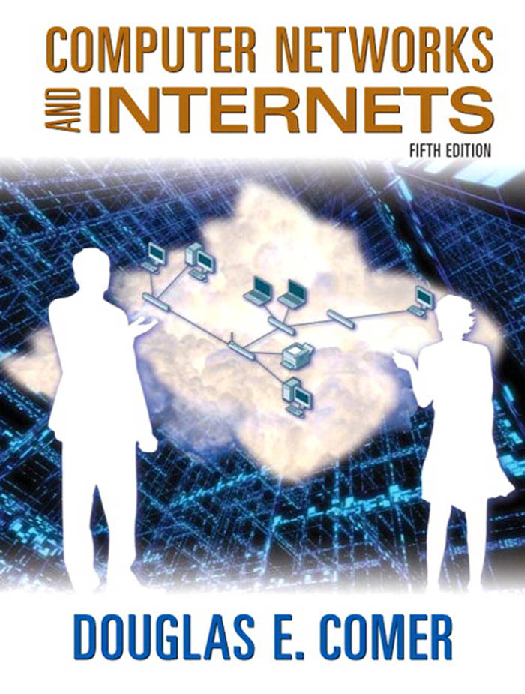
\includegraphics[width=0.8\textwidth,keepaspectratio]{figures/33.WirelessN/comer2008}
	\caption{Representation of data flow in a computer network. Adapted from \cite{comer2008}.}
	\label{fig:comer2008}
\end{figure}


\subsection{Current Wireless technologies and standards}
\label{subs:332}
The following sections will cover the wireless communications in smart metering systems, starting with the low-rate and low-power communications applied on smart meters and ending with the high-rate communications (and consequently higher costs and power than low rate communications). With the increasing on demand for higher bandwidth, broadband technologies such as mobile WiMAX, IEEE 802.16e and broadband \ac{PLC} are expected to be considered and used in newer installations, \cite{Mohassel2014}.


%As the demand for bandwidth increases, broadband technologies such as IEEE 802.16e, mobile WiMAX and broadband PLC are going to play a key role in newer installations, \cite{Mohassel2014}.

\subsubsection{IEEE 802.11 (\ac{WLAN} or Wi-Fi)}

IEEE 802.11 is the standard for the information exchange between systems and for the telecommunications. The coverage area of this technology is on local and metropolitan area networks (LANs and MANs). The specific requirements are on the Medium Access Control and on Physical Layer. The most popular versions of this standard is the IEEE 802.11b and IEEE 802.11g, that differs in the modulation technique (\ac{DSSS} technique versus  \ac{OFDM} modulation technique). The data rates are, respectively, 11 Mbps and 54 Mbps, \cite{Usman2013, ieee2012}.



\subsubsection{IEEE 802.15.4 (ZigBee)}

The standard IEEE 802.15.4 imposes conditions in the physical layer and media access control focusing on low-rate (up to 300 kHz) wireless personal area networks. Developed by the Zigbee Alliance and covering the specifications of the IEEE 802.15.4 on the physical layer and the medium access control, Zigbee is a commonly used for low power wireless communication technology. It operates on the \ac{ISM} bands of 868 MHz, 915 MHz and 2.4 GHz adopting \ac{DSSS}, \cite{Usman2013}.



\subsubsection{DASH7}

On the low-rate field of research, an alternative to Zigbee is the DASH7. Using the ISO/IEC 18000-7 standard to support this wireless sensor network technology, DASH7 is developed to reach active Radio Frequency Identification Devices (RFIDs) and operates at 433MHz band. The advantage is the typical range of 250m (could achieve 5 km) and has a typical and maximum data rates of 28 kbps and 200 kbps, being in this specifically designed for Smart Grid and for applications in Smart Energy.


\subsubsection{6LoWPAN}

This IETF development group promotes specifications for the usage of IPv6 on IEEE 802.15.4 networks. It allows the connection between low-power devices to \ac{IP} networks, with the usage of fragmentation and compression of messages. In conclusion, 6LoWPAN creates an adaptation layer between the IEEE 802.15.4 and IPv6.



\subsubsection{Wibree}

This wireless communication technology is designed for low power consumption and short-range communication. It is designed to work with Bluetooth and, the Bluetooth-Wibree depends on the existing Bluetooth RF and allows ultra-low power consumption.


\subsubsection{Industrial Wireless Communications: WirelessHART and ISA100.11a}

Launched by HART Communication Foundation in September of 2007, WirelessHART is an open wireless communication standard designated specifically for the process measurement and control applications, \cite{Song2008}. This standard is specifically designed to comply with industrial requirements, such as stricter timing requirement, higher security concern, immunity to harsher interferences and obstacles and enough scalability to be used in large process control systems.

Similarly, ISA100.11a aims to provide secure and reliable wireless communication for noncritical monitoring and control applications, \cite{Petersen2011}.





\subsubsection{IEEE 802.16 (WiMAX)}

On the field of the broadband wireless communication there is the Worldwide Interoperability for Microwave Access (WiMAX) under the IEEE 802.16 standard. It is specifically developed aiming the point-to-multipoint communications being applied in fixed and mobile applications and it has data rates up to 70 Mbps over a distance of 50 km. Framed into the smart grid systems, this communication technology is considered as a solution for high data rate communication link to be applied at the backbone of the utilities, \cite{Usman2013}.


\subsubsection{Broadband communications: GSM/GPRS and LTE/LTE-Advanced}

Operating at 900 MHz and 1800 MHz, the \ac{GSM} is the most used cellular network all over the world. The modulation technique is the \ac{GMSK} and it achieves transfer rates up to 270 kbps. Its architecture consists of four components: the Operation Support Substation, the Network Switching Substation, the Base Station Subsystem and the Mobile handset. Due to its level of development around the world being present in remote locations, this advantage makes this an interesting technology to be applied in \ac{SG} applications, \cite{Usman2013}.

\ac{LTE} is a recent standard for wireless technology that allows high data rates with high capacity and low latency and with a good \ac{QoS}. The improved version of this technology, the LTE-Advanced, admit higher capacity with expanded peak data rate of 1 Gbps for the downlink and 500 Mbps for the uplink, obtained on the increase of the spectral efficiency, higher  number of active subscribers connected at the same time, and better performance at cell edges, \cite{Mohassel2014}. This technology, for the smart metering environment where the high bandwidth and good \ac{QoS} are mandatory at some communication points.


\subsection{Protocols and standards}
%\lipsum[4]
\label{subs:333}
In computer networks, a protocol is a set of rules that ensure a communication of specific set of information between two machines. A standard is a document that specifies several aspects of something that has the overwhelming agreement and support of an entity (the standards making body). In the networking area, several protocols are supported by standards. In this section is presented some of the protocols that ensure a coherent communication among the sensor networks.

\subsubsection{IEEE 802.15}

The standard family defines the topologies and network roles. In particular, it defines the physical (frequency and channels, spectrum handling, modulation and bit rate) and \ac{MAC} (packet formats, operational modes, timing aspects, topologies) layers of the \ac{OSI} model, \cite{Hackmann2006}.


\begin{figure}[h!]
	\centering
	\includegraphics[width=1.05\textwidth,keepaspectratio]{figures/33.WirelessN/nancy2014}
	\caption{Members of the 802.15 family. Adapted from \cite{nancy2014} lecture presentation slides.}
	\label{fig:nancy2014}
\end{figure}

Based on figure \ref{fig:nancy2014}, the 802.15.4 is the standard that defines the \ac{PHY} and \ac{MAC} layers for low rate wireless personal area networks. It supports \textbf{full-function devices} (device capable of being the network coordinator or simple node and can have implemented complex network functionalities) and \textbf{reduced-function device} (limited devices with low-bandwidth limitations and limited or no-network intelligence). The possible network topologies are the following:

\begin{description}
	\item[Star ---] Each device in the network communicates with the full-function device network coordinator;
	
	\item[Peer-to-peer ---] All devices communicate with each other (if they are in the communication range). Sufficiently flexible to implement more complex topologies such as multi-hoping, cluster trees and mesh topologies;
	
	\item[Multi-hopping ---] This is a technique that allows the usage of two or more wireless nodes to convey data from a source to a destination;
	
	\item[Cluster trees] Topology to reduce the routing complexity where each node knows its parent node and all its child nodes. It has always only one single path between two nodes.
	
	\item[Wireless mesh] This technique allows data to be propagated along a path by hopping from node to node until it reaches its destination.
	
\end{description}

\subsubsection{802.15.4-based wireless standards}

Radmand et al. (2010) presents a comparison of wireless sensor standards for industrial applications, \cite{Radmand2010}. In figure \ref{fig:radmand2010} is present the overall schema of the wireless standards.


\begin{figure}[h!]
	\centering
	\includegraphics[width=0.6\textwidth,keepaspectratio]{figures/33.WirelessN/radmand2010}
	\caption{Overall schema of wireless standards. Adapted from \cite{Radmand2010}.}
	\label{fig:radmand2010}
\end{figure}


\subsection{Communication \ac{KPI}}
%\lipsum[4]
\label{subs:334}
According to Radmand et al. (2010), it is identified the following "Industrial Requirements" for the WSN's, \cite{Radmand2010}:

\begin{description}
	\item[Reliability ---] Reliability is a measurement of the transmission accuracy, in percentage, that evaluates the amount of data that reach its destination. This measurement uses the properties of data communication, acknowledge-based usually.
	
	\item[Latency ---] Latency is the measurement of the time delay and is defined as the time that a data packet takes to be transmitted from the source to the destination. The latency is directly related to the link quality and a high latency link is result of a link with high signal-to-noise ratio. 
	
	\item[Sensor Data Update Rates ---] This \ac{KPI} is not directly related with the communication link. However, the update rate of the sensor data affects the power consumption due to the increase of the processing effort. In a SYNC-based update rate, this \ac{KPI} is related to the frequency of the SYNC event.
	
	\item[Wireless Transmission Range ---] This \ac{KPI} is the maximum distance that a communication link supports the data transfer with a given reliability and in specific conditions (indoor/outdoor; line-of-sight (LOS)).
	
	\item[Power consumption ---] The power consumption is a measurement of the combination of the computational effort of the nodes and the transmission effort. It is directly related with the update rate as well as with the link quality and, if it exists, the routing activity in each node.
	
\end{description}

%\subsection{Emerging Technologies and Research Trends}

%%ver livro khan

\subsection{Network Simulators and Network Emulators}
\label{subs:335}

In this subsection is covered the network simulators. The usage of network simulators allows the modeling of various scenarios of real environment. However, pure network simulators avoid the interaction with real environment, which leads space for network emulators, as a hybrid method to combine simulation capabilities with hardware and software components of real networks. Therefore, in this subsection is referred the simulators that allows integration with hardware and software network components, to have an overview on the network emulators.

In figure \ref{fig:simul_VS_emul} is presented the framework on the mechanisms to evaluate the performance of networks.

\begin{figure}[h!]
	\centering
	\includegraphics[width=1\textwidth,keepaspectratio]{figures/33.WirelessN/simul_VS_emul}
	\caption{Simulation \& emulation framework.}
	\label{fig:simul_VS_emul}
\end{figure}

An extensive review on simulation tools, made by \cite{nayyar2015}, is presented as following:

\begin{description}
	\setlength\itemsep{0.5em}
	%%1
	\item [NS-2 (network simulator-2)] 
	Object orientated discrete event simulator tool, based on two languages (C++ and OTcl). 
	
	%%2
	\item [NS-3 (network simulator-3)] 
	Written in pure C++, this simulator has been extensively explored in the literature with various modules like 802.15.4, 6LoWPAN and RPL available. With the usage of ns-3 in emulation mode, the implementation of real testbeds can be validated since it is possible to generate repeatable experimental results, with the usage of real-world network environment that includes all of the ns-3 tracing, logging, visualization and statistics gathering tools.
	
	%%3
	\item [OMNET++] 
	This simulator is based in C++ in the basic modules and uses Network DEscription (.NED) scripts to connect and assemble the simulation basic modules.

	%%4
	\item [J-Sim] 
	JavaSim Simulator has been developed in Java and it has several advantages to carry out large scale WSN simulations.

	%%5
	\item [Mannasim] 
	Is based on NS-2 to perform WSN simulations.

	%%6
	\item [SensorSim] 
	Similarly to Mannasim, this is a framework for WSN based on NS-2 simulator. However, currently it is not available to the public. 

	%%7
	\item [NRL Sensorsim] 
	This extension to NS-2 simulator is focused on WSN, similarly to SensorSim and Mannasim frameworks. Currently, it is no longer in development and does not have support.

	%%8
	\item [NCTUns 6.0] 
	On the field of network emulators, this software has the main advantage of using the real world Linux TCP/IP stack and implements almost every IEEE network standards. Last release was on 2010.

	%%9
	\item [SSFNet] 
	Java simulator designed especially for WSN's. Last release in 2004.

	%%10
	\item [GloMoSim] 
	Non-commercial simulator (the commercial version is \textit{"QualNet"}) designed for wireless and wired network systems.

	%%11
	\item [QualNet 7.0 + EXata 5] 
	Considered one of the most advanced simulator platform these days, QualNet enables a high fidelity virtual model of network, with an advanced GUI. It has a free academic version.

	%%12
	\item [sQualNet Simulator] 
	Is an extension of QualNet for sensor network specific models. 

	%%13
	\item [OPNET Modeler Suite] 
	Is a powerful collection with an interactive GUI to build network scenarios. It has a free academic edition. 

	%%14
	\item [SENSE] 
	Is a powerful sensor network simulator and emulator.

	%%15
	\item [DRMSim] 
	Is a Java-based software that enables large-scale network simulation.

	%%16
	\item [NetSim] 
	Is a simulator designed for protocol modeling, network research and development and defense applications.

	%%17
	\item [UWSim] 
	This simulator is designed for marine robotics research.

	%%18
	\item [Visual Sense] 
	This modeling and simulation software is designed for wireless and WSN applications, as an extension of Ptolemy II.

	%%19
	\item [Viptos] 
	Is an interface/bridge between TinyOS and Ptolemy II.

	%%20
	\item [PTOLEMY II] 
	Is an open source simulation software, based on Java and with actor-oriented design (where actors are software components, have a concurrent execution and communicate via interconnected ports)
	
	%%21
	\item [SENS] 
	This specific framework for WSN's simulator and emulator that uses a simplified sensor model.
	
	%%22
	\item [SHAWN]	
	Is a customizable sensor network simulator focused on the simulation of the effect caused by a phenomenon (not the phenomenon itself) with scalability and support for extremely large networks. According to SHAWN development repository, last contribution was on 2013.
		
	%%23
	\item [SIDnet-SWANS]
	This Java-based simulator was made to provide a simulation and proof-of-concept platform for application of WSN's.
	Latest version was released in 2011.
	
	%%24
	\item [WSim/Worldsens Simulator/WSNet Simulator]
	This simulator states for being an event-driven simulator for large scale wireless networks. Latest version was released in 2009.

	%%25
	\item [WSN Localization Simulator]
	This is a WSN location simulator stating for being easy, scalable and extendable to many/different localization schemes. It was released in 2013.
	
	%%26
	\item [NetTopo Simulator]
	This framework is an open source simulator designed in Java. Its main objective is to analyze various algorithms in WSN's. 
	
	%%27
	\item [SIDH]
	Is a Java-based simulator focused on the simulation of thousands of sensor nodes.
	
	%%28
	\item [PROWLER]
	The Probabilistic Wireless Sensor Network Simulator is a framework that runs under Matlab and is focused to TinyOS applications.
	
	%%29
	\item [Matlab/Simulink]
	With extensive usage by the research community, Matlab and Simulink software provides resourceful toolboxes for simulation of communication networks, being possible to build a complete WSN model system.
	
	%%30
	\item [PiccSIM]
	This simulation platform uses Matlab/Simuling and NS-2 for networked control systems (in particular wireless)
	
	%%31
	\item [LabVIEW]
	Various toolboxes to simulate WSN's are available with LabVIEW.
	
\end{description}


\subsubsection{Evaluation of network tools}

In the previous list, several tools for the evaluation of network performance was presented. Special attention is given for the tools that has large support either for implementation of several network technologies (wired and wireless) and, with this requirement, the following network simulators will be considered for further research:
	
\begin{itemize}
	\setlength\itemsep{-0.5em}
	\item NS-3;
	\item OMNET++;
	\item QualNet 7.0 + EXata 5;
	\item MatLab Simulink;
\end{itemize}




\newpage




\section{Section 4: Smart metering}

In this section, special attention is given to smart metering. The smart grid framework is presented to justify the need for smart meters and then, an overview on the features of metering systems is presented.
This section is concluded with the presentation of the metering systems in railways.

%1.	Smart grids and the need for smart meters

%2.	Metering systems – overview

%3.	Metering systems in railways

%4.	Wireless sensor networks – overview

%5.	Smart metering with WSN in Railway Transportation System (RTS)

\subsection{Smart grids and the need for smart meters}

Smart Grids improves the functionality and concept of traditional electrical grids by obtaining the grid component's data using Information and Communication Technology (ICT). Such grids benefit the reliability and the efficiency of the system with the usage of the acquired data, \cite{Mohassel2014}.

Although the smart meters does not have an effective definition, those devices are composed by an electronic box and a communication link, \cite{Seppo2012}. A smart meter is responsible for measuring the energy-related parameters and the user consumption with a given time interval. All those measurements are then transmitted upon a communication network to the utility or to other player with the responsibility of using the meter data. The information obtained from the data is shared with consumer-side devices, to inform the end-users on their related costs and energy usage, \cite{Siano2014}.

Smart meters implement a bidirectional communication on top of AMR. They are inherent to smart grid systems. 

Similarly to the evolution of electricity meters, the utility grid has evolved from a centralized production and control perspective to a distributed one. The conventional electrical grid is a network with a transmission link connecting power producers and end-user consumers. The control and distribution of electrical power is made in a centralized way. With the increase of power demand, increase of complexity and having more and more decentralized power generation, a migration to the smart grid framework is required, \cite{Reddy2014}.

\subsection{Features of Smart Meters and metering systems}

A smart metering system combines several controlling devices, a extensive number of sensors for measuring the parameters and devices responsible for the transferring of the data and the commands. The detection of unauthorized consumption due to electrical energy theft and the improvement of the energy in the distribution are other advantages of smart meters. These devices acts as a gateway by having a communication interface protocol to the database stored by the utility company, \cite{Reddy2014}.

The design of an ideal smart grid has to focus on prediction, adaptability and reliability points. Moreover, it requires to cover the demand adjustment, the load handling, flexibility and sustainability and it should incorporate advanced services. In advance, an end to end control capability has to be ensured as well as finding the optimal cost and asses, increase the quality of energy and quality of service. Another features of smart grids are the automatic restoration ans self-healing, being all the previously presented features of the smart grids highly dependent of the role of the smart meters, \cite{Mohassel2014}.

Smart-meter types are also distinguished based on features like data-storage, communication type and connection with the energy supplier. The data storage capability allows data to be stored in the meter, being transferred after a few days or weeks to the Meter Data Management System (MDMS) of the utility. Compensations for some power quality deficiencies can be also considered; therefore the future meters should be also capable of register certain basic power quality characteristics. In advance, the design of rate and tariffs of electricity providers determine the requirements such as the period of meter intervals or the temporal resolution (commonly ranging from 15 min to 1 h). During those intervals, the production and consumption of active and reactive power is mandatory to be separately measured, \cite{Siano2014}.

\subsection{Metering systems in railways}

Towards na increase of interoperability of the rail system within the Community \cite{eur-lex2008}, the Directive 2008/57/EC specifies the need of Technical Specifications for Interoperability (TSIs), presenting essential requirements in which each rail subsystem should meet to ensure the interoperability of the railway system within the EU. Those TSIs are of the responsibility of European Union Agency for Railways (ERA) and are listed as following:

\begin{itemize}
	\setlength\itemsep{-0.5em}
	\item Locomotives and passenger rolling stock - 1302/2014;
	\item Noise - 1304/2014;
	\item Wagons - 321/2013;
	\item Infrastructure - 1299/2014/EU;
	\item Energy - 1301/2014;
	\item Control command and signalling - 2012/88/EU;
	\item Persons with reduced mobility - 1300/2014/EU;
	\item Safety in railway tunnels - 1303/2014;
	\item Operation and traffic management - 2015/995/EU;
	\item Telematics applications for freight service - 1305/2014/EU;
	\item Telematics applications for passenger service - 454/2011;
		
\end{itemize}


On the energy field and with the purpose of implementing on-ground energy data collecting systems (data collecting service - DCS), technical specifications for interoperability relating to the ‘energy’ subsystem of the rail system in the Union are specified in the Commission Regulation (EU) No 1301/2014, \cite{eur-lex2014}. 



The On-Board energy measurement systems are pointed in Appendix D of Commission Regulation (EU) No 1302/2014 \cite{eur-lex2014b}. This regulation appendix presents the requirements for such energy measurement system. The general architecture is defined as following:

\begin{itemize}
	\setlength\itemsep{-0.5em}
	\item \textbf{Energy measurement function (EMF)}, measuring the voltage and current, calculating the energy and producing energy data;
	\item \textbf{Data handling system (DHS)}, producing compiled energy billing data sets for energy billing purposes, by merging data from the EMF with time data and geographical position, and storing it to be sent to on-ground data collection system (DCS) by a communication system;
	\item \textbf{On-board location function}, giving geographical position of the traction unit. Contrary to fixed installation revenue meters, train meters must have the knowledge of time and geographical position \cite{metas2015};
\end{itemize}

Figure \ref{fig:EMS} presents the general overview of the on-board energy measurement system.

\begin{figure}[h!]
	\centering
	\includegraphics[width=\textwidth,keepaspectratio]{figures/34.SmartM/EMS}
	\caption{Functions, data flow and regulation scope of on-board energy measurement system.}
	\label{fig:EMS}
\end{figure}

As global requirements, all active and reactive energy should be measured, the measurement equipments should be rated to match the traction unit current and voltage rating, the system should be protected from intrusion, and finally, the loss of power in the  measurement system should not affect the data stored in EMS.

Complementary to the previously presented system requirements, each component of the energy measurement system has specific requirements as listed as following:

\begin{description}
	\setlength\itemsep{-0.5em}
	
	\item [Energy measurement function (EMF)] Has specific metrological requirements to specify the accuracy of the sensors and it has the requirement of having the reference period of 5 minutes defined by the UTC clock time (shorter measuring period is allowed in the case that the data is aggregated into 5 minutes time reference period);
	
	\item [Data handling system (DHS)] Should compile the data (without corrupting them), using the same time reference as EMF. This system should store compiled data of, at least, 60 days' continuous work and should have an alternative method of accessing the data. Finally, this system should produce compiled energy billing data sets (CEBD) by including an EMS identification number, a timestamp, a location data and the consumed/regenerated active and reactive energy.
	
	\item [Location function] Has specific location requirements to define the latitude and longitude, as well as a accuracy of 250m and the location data information should have the same timestamp.
	
	\item [On-board to ground communication] The specification related to interface protocols and transferred data format are an open point.
	
\end{description} 


 \cite{metas2015} identifies the EN 50463 that should be considered to the certification of Energy Measurement Systems on on-board trains. This standard is divided in 5 areas as presented in figure \ref{fig:gatti2011}.
 
% \begin{description}
% 	\setlength\itemsep{-0.5em}
%	\item [EN 50463-1] General;
%	\item [EN 50463-2] Energy Measurement Function;
%	\item [EN 50463-3] Data Handling System;
%	\item [EN 50463-4] Communication;
%	\item [EN 50463-5] Conformity Assessment.
% \end{description} 



\begin{figure}[h!]
	\centering
	\includegraphics[width=\textwidth,keepaspectratio]{figures/34.SmartM/gatti2011}
	\caption{Structure of Energy Measurement System (EMS) EN 50463 standard. Adapted from \cite{gatti2011}}
	\label{fig:gatti2011}
\end{figure}


%\subsection{Wireless sensor networks – overview}


%\subsection{Smart metering with WSN in Railway Transportation System (RTS)}


%%%%%%%%%%%%%%%%%%%%%%%%%%%%%%%%
%%%%%%%%%%%%%%%%%%%%%%%%%%%%%%%%%
%%%%%%%%%%%%%%%%%%%%%%%%%%%%%%%%%
\newpage




\section{Decision Support Systems}
In previous chapters we have presented the \ac{RTS} and the means to acquire energy information of such system.
In this chapter we denote the possible generation of knowledge that can help to feedback the \ac{RTS} in a  \ac{DSS}.

In subsection \ref{subs:351} we present the framework that supports the \ac{DSS}. In further subsections we display some \ac{DSS} that contributes to the increase of energy efficiency in railways.

%1.	Overview/definition
%2.	Eco-driving – driving assistant
%3.	Timetable scheduling
%4.	Maintenance support

\subsection{The information and knowledge as the base of \ac{DSS}}
\label{subs:351}

	At a lower level of a data acquisition system, the measurements of needed variables are performed. 
	Combined, this raw data supports the generation of information.
	In the field of energy data acquisition system, the information is the combination of the voltage/current electric measurements and non-electric data (such as location, timestamp, etc.).
	
	This information can be stored in databases and, with this accumulated information, it is possible to extract knowledge on the energy flow in \ac{RTS}.
	This knowledge is the base of \ac{DSS}. For instance, a railway operator that has the knowledge that a particular action results in energy efficiency increase/decrease can actively contribute to a better usage of \ac{RTS} resources.
	
	The \ac{DSS} can be used in other areas rather than energy efficiency. 	
	Several DSS are used for various areas of \ac{RTS} operation, either for immediate and long-term decision support.
	As examples, the literature presents the works on traffic control support and dynamic re-scheduling \cite{dariano2009, krasemann2012}, crew planning \cite{freling2004}, strategic railway capacity planning \cite{lai2011} and the work on track maintenance and renewable management \cite{guler2013}.
	
	
	In the scope of this work, special attention will be given to \ac{DSS} that contribute to the increase of energy efficiency. In order to decrease the energy consumption, Scheepmaker et al. (2017) identifies two ways: (1) the \ac{EETC} or eco-driving, that uses the least amount of energy for a given timetable and (2) the \ac{EETT}, that constructs the timetable with the objective of reducing the energy consumption,\cite{scheepmaker2017}.
	
\subsection{Eco-driving – driving assistant}
\label{subs:352}

	This type of \ac{DSS} is directly related to the decrease of energy consumption. This topic is inserted in the field of operational research and is based on the optimal control theory, where the train optimal control is derived from Pontryagin's maximum principle, \cite{pontryagin1963}.  
	In synthesis, the determination of optimal speed profile will define the best traction regimes for each condition. The traction regimes are shown in figure \ref{fig:scheepmaker2017a} and described as following:
	
	\begin{itemize}
		\setlength\itemsep{-0.5em}
		\item Acceleration with maximum available traction force;
		\item Cruising, as the traction regime that keeps the velocity constant;
		\item Coasting, where the free train movement due to inertia defines the traction regime;
		\item Full braking, used to reduce the train to a desired speed or fully stop the train, and a moment where the energy can be regenerated;
	\end{itemize}
	
	\begin{figure}[h!]
		\centering
		\includegraphics[width=0.5\textwidth,keepaspectratio]{figures/35.DSS/scheepmaker2017a}
		\caption{Optimal traction regimes. Adapted from \cite{scheepmaker2017}.}
		\label{fig:scheepmaker2017a}
	\end{figure}
	
	

\subsection{Timetable scheduling}
\label{subs:353}

	Similarly to Eco-driving \ac{DSS}, in this type of \ac{DSS} is addressed the minimization of the energy consumption, with three research streams in the literature: (1) the usage of the total running time of a train as a variable, (2) the optimal distribution of running time supplements over successive train runs and (3) the synchronization of the timetables to maximize the usage of regenerated braking energy, \cite{scheepmaker2017}.
	
	
	
%\subsection{Maintenance support}
%\label{subs:354}

\newpage






\section{Section 6: Outlier detection in RTS energy measurement}


1.	Definition of outlier detection in RTS energy measurement perspective
2.	Literature review of Outlier detection in WSN
a.	Motivation
b.	Research areas
c.	Challenges
3.	Taxonomy of outlier detection techniques
a.	Classification based
b.	Statistical based
c.	NN-based
d.	Clustering based
e.	Spectral decomposition-based

%\chapter{Results and Discussion}
%\input{chapters/4.Results}

\chapter{Methodology and Work Plan}
%\lipsum[4-4]

This chapter presents the methodology that is intended to be adopted in the development of this PhD thesis. Based on the methodology and expected contributions, a work plan for the upcoming years is presented.

In section \ref{sec:41} is presented an overview of the architecture of proposed work. In sections \ref{sec:42} and \ref{sec:43}, the methodology and expected contributions are detailed.
In section \ref{sec:44} is presented the workplan.

\section{Architecture of proposed work}
\label{sec:41}


Framed in this PhD work, a smart metering system can be divided in four major areas, as represented in figure \ref{fig:41topLevel}. On lower level, the needed data is \textbf{measured} (such as voltages, currents and so on).
Based on this measurements, \textbf{information} can be obtained (such as power, energy, power factor, GPS location).
This information can be stored in databases and, a further step is on the analysis of this information towards obtaining \textbf{knowledge} that can be used in a \textbf{Decision Support System} (DSS).

\begin{figure}[h!]
	\centering
	\vspace{-1em}
	\includegraphics[width=0.3\textwidth,keepaspectratio]{figures/4.Method/pyramid}
	\caption{Overall functional architecture of a smart metering system.}
	\label{fig:41topLevel}
\end{figure}

This work will focus on the two lower levels of the smart metering system pyramid. 
Therefore the energy data must be acquired, processed, transmitted and stored in a centralized database, as represented in figure \ref{fig:41dataFlow}.

\begin{figure}[h!]
	\centering
	\includegraphics[width=0.8\textwidth,keepaspectratio]{figures/4.Method/data_flow}
	\caption{Data flow of measurement-information layers.}
	\label{fig:41dataFlow}
\end{figure}


A distributed sensor network to perform the acquisition of the energy measurements in each of the transformer's secondary windings is, at this moment, of advanced interest.
For the acquisition part, a non-intrusive self-powered sensor node will be considered.
The processing part depends on an accurate knowledge of the modeling parameters of the catenary and the traction transformer, which depends on train GPS location and power flow conditions. 
It is expected that each of the sensor node contributes to this processing part.
These two parts are further detailed in the methodology and expected contributions of section \ref{sec:42}.

%The definition of the processing part will validate if the proposed acquisition architecture has enough support.

% At this moment a solution with only a current sensor, for the acquisition in each transformer's secondary, is of advanced interest. 

The transmission of the generated information to a centralized storage is further detailed in section \ref{sec:43}. Several models will be considered for accurate simulation of such transmission network. The overall architecture of the system is presented in figure \ref{fig:41architecture}.

\begin{figure}[h!]
	\centering
	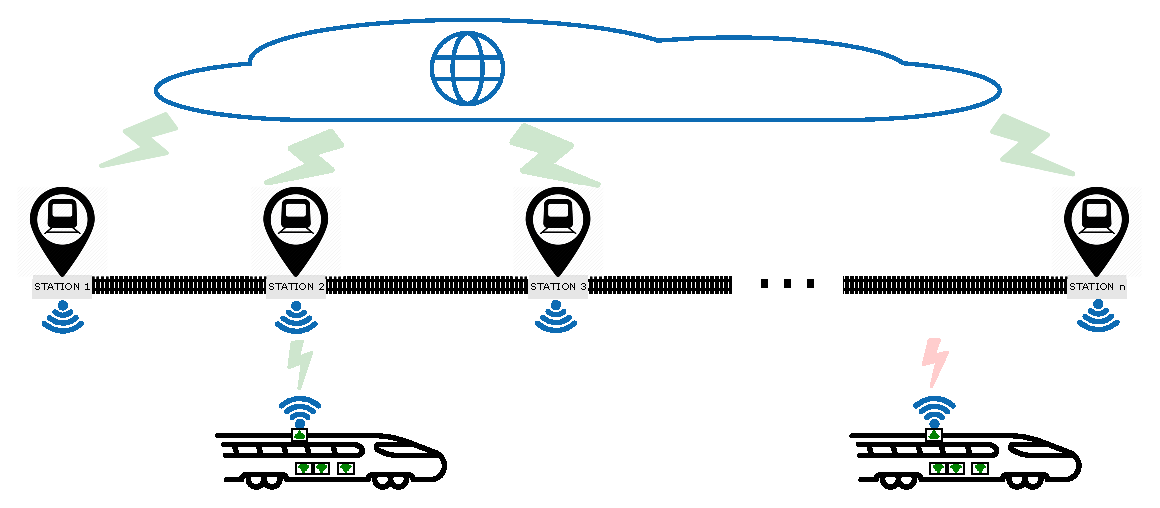
\includegraphics[width=1.0\textwidth,keepaspectratio]{figures/architecture}
	\caption{Architecture of proposed work.}
	\label{fig:41architecture}
\end{figure}







%%%%%%%%%%%%%%%%%%
%%%%%%%%%%%%%%%%%%
%%%%%%%%%%%%%%%%%%
%\newpage
\section{Non-intrusive self-powered sensor node}
\label{sec:42}
\subsection{Purpose}

The purpose of this section is to cover the acquisition and processing parts of the data-flow presented previously. As a starting point, a non-intrusive and self-powered sensor node allows the measurement of AC currents in all transformer secondary windings, as illustrated in figure \ref{fig:4.powerSensing}. This figure is based on the 3400 series train topology of \textit{Comboios de Portugal} (CP) used in urban services.

Based on the field measurements, a data concentrator will receive the current and voltage measurements from each sensor node. This data concentrator generates information based on the needed estimations and the acquisition of GPS location, as proposed by the European Commission regulation No 1301/2014. For each time-stamp, the active and reactive power is calculated and transmitted together with the geographical position.

In the scope of Shift2Rail, is expected to develop a smart metering system for RTS. Assuming that a non-intrusive measurement system is of extreme interest, this proposal of a non-intrusive and self powered sensor node goes along the goals of Shif2Rail.

On the field of measurement, non-intrusive technical solutions has been used for several years for current measurement, such as hall-effect current sensors, rogowsky probes or current transformers.
For self-powering purposes, some studies on using current transformers for energy harvesting has been proposed in the literature (\cite{ahola2008}, \cite{wu2013}, \cite{moon2015}, \cite{amaro2015}, \cite{brunelli2016}).


\begin{figure}[h!]
	\centering
	\vspace{-1em}
	\includegraphics[width=0.7\textwidth,keepaspectratio]{figures/4.Method/powerSensing}
	\caption{Power architecture of case-study train.}
	\label{fig:4.powerSensing}
\end{figure}






\subsection{Methodology}

The methodology is divided into two parts. The first part will be related to the processing of the data generated by the sensor nodes and the second part is the definition of the sensor itself.

As a starting point of the methodology, it is expected to work on the \textbf{development of models using simulation frameworks} similar to the ones presented in figure \ref{fig:4.methodElectrical}. The modeling of such architecture allows the evaluation of the power contribution of a train, at a certain instant, to the power injected to the catenary. This methodology will contribute to \textbf{simulation and implementation of processing algorithms} in the train data concentrator that, based on the measurement of AC secondary winding's voltages and currents, will generate the accurate value of the energy injected in the catenary by the traction substation. The expected result will be the comparison and validation of the energy injected into the catenary (retrieved from the traction substation meter) and the estimated energy (as the outcome of this part of work).
%The expected result will be the comparison between the estimation and the measured injected energy in the catenary.

In this second part of the methodology, or the acquisition part, the sensor will be defined and validated. As a first step in the methodology, using Ansys or similar Finit Element Method (FEM) software, the \textbf{current and electric field of one winding will be simulated}. With the results of this simulation, the current and voltage sensors will be evaluated. In a further step, \textbf{real experiments on low voltage test-bench} will test the proposed sensor node.



\begin{figure}[h!]
	\centering
	\includegraphics[width=0.9\textwidth,keepaspectratio]{figures/4.Method/methodElectrical}
	\caption{Models needed for simulation.}
	\label{fig:4.methodElectrical}
\end{figure}



\subsection{Simulation tools and frameworks}

\cite{pilo2000} identifies the need of two tools for the simulation of railway power lines: (1) the simulator for the railway line and (2) an electrical system simulator. Based on that, \cite{almagro2017} uses the simulation tool \textbf{OpenDSS} with the Python integration for the simulation of the railway power lines. A further study on OpenDSS shows enough documentation and recent updates (march 2017) with the possible integration with VBA Excel, MatLAB and Python scripts.

Mathworks suggests also the usage of \textbf{MatLAB and Simulink} for rail electrical systems modeling. 
Similarly, \textbf{Ansys} products are suggested for the simulation of railway power systems as well as \textbf{PSIM}. The three previously presented products are also flexible to work in co-simulation, with the advantage of choosing the best software for the most straightforward application.


	\subsection{Contributions}
	
	On the energy measurement and information generation of the sensor nodes, two contributions can be considered as follows:
	
	\begin{itemize}
		\setlength\itemsep{0em}
		
		\item \textbf{New energy metering architecture}, according to some specifications such as the usage of a non-intrusive approach.
		This architecture will generate energy information about the powerflow of the railway system.
		
		\item \textbf{Accurate estimation of power flow} into catenary, based on on-board measurements. The available parameters will be: (1) the RMS voltage, current and apparent power, (2) the instantaneous active power, reactive power, power factor and frequency, and (3) the cumulative energy consumptions in terms of kVAh, kVARh and KWh.
		
		
	\end{itemize}

%	\begin{itemize}
%		\setlength\itemsep{0em}
%		\item New energy metering architecture using a non-intrusive approach.
%		
%		\item Accurate estimation of injected power into catenary, that is needed for train operation, based on on-board measurements.
%		
%	\end{itemize}
	
%%%%%%%%%%%%%%%
%%%%%%%%%%%%%%%
%%%%%%%%%%%%%%%

\section{RTS wireless network}
\label{sec:43}

\subsection{Purpose}

The main purpose of the RTS wireless network is to transmit energy measurements and information generated by the nodes to a centralized storage server. 

As a lower level and as previously presented, each train has current sensors as nodes and a data concentrator. Between nodes and data concentrator, AC voltage and current measurements must be exchanged.
At this level, the relevant issue will be the presence of EMI, that will affect the communication link.

Between train data concentrator and ground-level, the train movement should be considered to better comply with the purpose of transmission the information generated at trains to the centralized storage server. 

Further modeling and simulation of a WSN for energy measurement of RTS rolling stock will be made.



\subsection{Methodology}

The methodology for this part will include the \textbf{modeling and simulation} of network blocks similar to the ones presented in figure \ref{fig:4.methodWireless}. An accurate modeling and simulation will define the more appropriate network technologies to implement in this RTS network. 
The simulation will be performed in a NS-3 simulator or similar.
The \textbf{results} of such simulation will define the max data-rate of the sensor nodes as well as the nodes energy consumption required for the information transmission.

\begin{figure}[h!]
	\centering
	\includegraphics[width=0.9\textwidth,keepaspectratio]{figures/4.Method/methodWireless}
	\caption{Models needed for simulation.}
	\label{fig:4.methodWireless}
\end{figure}

\subsection{Simulation tools and frameworks}

Several simulators/emulators were presented in the literature review chapter. From those, special attention is given to the NS-3 simulator and the MatLAB/Simulink tool.  
%<<necessário avaliar melhor os restantes candidatos>>


\subsection{Contribution}
%An energy measurement system in rolling stock does not require a broadband real-time/continuous communication (such as LTE), being possible to collect and store data in train data concentrator and, while the train is waiting at station for passenger exchange (which lasts for less than one minute), the data is transferred between train and station AP (and then to a remote server). Therefore, the contribution will be the cost reduction of information transmission of energy sensor network data

Regarding the energy information transmission and storage into centralized database, the following contributions are expected:

\begin{itemize}
	\setlength\itemsep{0em}
	
	\item \textbf{Availability of measured data} from trains where currently limited/inexistent energy measurement is performed.
	
	\item Data-rate increase of energy measurements, which will result on direct \textbf{increase on the quality of information of energy}. This increase will overcome the 5 minute data-rate that currently are used in energy meters.
	
\end{itemize}

A further contribution can be the reduction of the dependence of broadband real-time/continuous communication (such as LTE), with the direct cost reduction of information transmission of energy RTS data.

%\begin{itemize}
%	\setlength\itemsep{0em}
	
%	\item As a starting point, one contribution will be the availability of measured data from trains where currently no energy measurement is performed.
	
%	\item A second contribution will be the data-rate increasing of energy measurements, which will result on direct increase on the quality of information of energy.
	
%	\item A further contribution can be the avoidance of broadband real-time/continuous communication (such as LTE), being possible to collect and store data in train data concentrator and, while the train is waiting at stations, the data is transferred between train and station AP (and then to a remote server). A possible contribution will be the cost reduction of information transmission of energy sensor network data.
%\end{itemize}

\newpage
\section{Work plan}
\label{sec:44}

Based on the before-mentioned objectives, an annual planning for future developments was built for the next three years. 
The work plan is presented in Table \ref{workplan}. 


Secondary tasks of the work plan are the deliverables for the iRail programme and for the FCT institution, which occurs at end of academic year. 

% Please add the following required packages to your document preamble:
% \usepackage{booktabs}
% \usepackage{multirow}
\begin{table}[htbp]
	\centering
	\caption{Thesis work plan}
	\label{workplan}
	\footnotesize
	\setlength\extrarowheight{2pt}
	\resizebox{1.0\textwidth}{!}{ 
	\begin{tabular}{ccccc}
		\hline
%		\hline
		\textbf{Year}                            & \textbf{Semester}                         & \multicolumn{2}{c}{\textbf{Task}}                                                                                                                                                                                                                                                & \textbf{Milestone}                                                                                                  \\ \hline \hline
		\multicolumn{1}{|c|}{\multirow{6}{*}{1}} & \multicolumn{1}{c|}{\multirow{3}{*}{1st}} & \multicolumn{1}{c|}{\multirow{2}{*}{Train power model development}}                                                                      & \multicolumn{1}{c|}{\begin{tabular}[c]{@{}c@{}}Simulation of \\ traction power transformer\end{tabular}}                              & \multicolumn{1}{c|}{}                                                                                               \\ \cline{4-4}
		\multicolumn{1}{|c|}{}                   & \multicolumn{1}{c|}{}                     & \multicolumn{1}{c|}{}                                                                                                                    & \multicolumn{1}{c|}{\begin{tabular}[c]{@{}c@{}}Simulation of \\ train power system\end{tabular}}                                      & \multicolumn{1}{c|}{}                                                                                               \\ \cline{3-4}
		\multicolumn{1}{|c|}{}                   & \multicolumn{1}{c|}{}                     & \multicolumn{1}{c|}{\multirow{3}{*}{RTS energy model development}}                                                                       & \multicolumn{1}{c|}{Integration with real case-study}                                                                                 & \multicolumn{1}{c|}{}                                                                                               \\ \cline{2-2} \cline{4-4}
		\multicolumn{1}{|c|}{}                   & \multicolumn{1}{c|}{\multirow{3}{*}{2nd}} & \multicolumn{1}{c|}{}                                                                                                                    & \multicolumn{1}{c|}{\begin{tabular}[c]{@{}c@{}}Simulation of \\ railway power system\end{tabular}}                                    & \multicolumn{1}{c|}{}                                                                                               \\ \cline{4-4}
		\multicolumn{1}{|c|}{}                   & \multicolumn{1}{c|}{}                     & \multicolumn{1}{c|}{}                                                                                                                    & \multicolumn{1}{c|}{Algorithm implementation}                                                                                         & \multicolumn{1}{c|}{}                                                                                               \\ \cline{3-4}
		\multicolumn{1}{|c|}{}                   & \multicolumn{1}{c|}{}                     & \multicolumn{1}{c|}{\multirow{2}{*}{\begin{tabular}[c]{@{}c@{}}Energy measurement system:\\ node development\end{tabular}}}              & \multicolumn{1}{c|}{\begin{tabular}[c]{@{}c@{}}Hardware development of\\ Energy Measurement Node\end{tabular}}                        & \multicolumn{1}{c|}{}                                                                                               \\ \cline{1-2} \cline{4-5} 
		\multicolumn{1}{|c|}{\multirow{6}{*}{2}} & \multicolumn{1}{c|}{\multirow{3}{*}{1st}} & \multicolumn{1}{c|}{}                                                                                                                    & \multicolumn{1}{c|}{\begin{tabular}[c]{@{}c@{}}Results acquisition: \\ test bench validation of\\ Energy Measurement Node\end{tabular}} & \multicolumn{1}{c|}{\begin{tabular}[c]{@{}c@{}}Publication(s):\\ Energy Measurement Node\end{tabular}}                 \\ \cline{3-5} 
		\multicolumn{1}{|c|}{}                   & \multicolumn{1}{c|}{}                     & \multicolumn{1}{c|}{\multirow{3}{*}{\begin{tabular}[c]{@{}c@{}}RTS wireless smart \\ metering network\\ model development\end{tabular}}} & \multicolumn{1}{c|}{Model simulation}                                                                                                 & \multicolumn{1}{c|}{}                                                                                               \\ \cline{4-4}
		\multicolumn{1}{|c|}{}                   & \multicolumn{1}{c|}{}                     & \multicolumn{1}{c|}{}                                                                                                                    & \multicolumn{1}{c|}{Integration with real case-study}                                                                                 & \multicolumn{1}{c|}{}                                                                                               \\ \cline{2-2} \cline{4-5} 
		\multicolumn{1}{|c|}{}                   & \multicolumn{1}{c|}{\multirow{3}{*}{2nd}} & \multicolumn{1}{c|}{}                                                                                                                    & \multicolumn{1}{c|}{\begin{tabular}[c]{@{}c@{}}System integration with \\ energy measurement nodes\end{tabular}}                      & \multicolumn{1}{c|}{\begin{tabular}[c]{@{}c@{}}Publication(s): \\ RTS wireless \\ smart metering network\end{tabular}} \\ \cline{3-5} 
		\multicolumn{1}{|c|}{}                   & \multicolumn{1}{c|}{}                     & \multicolumn{1}{c|}{\multirow{3}{*}{System integration}}                                                                                 & \multicolumn{1}{c|}{\begin{tabular}[c]{@{}c@{}}Development of energy data\\ storage system;\end{tabular}}                             & \multicolumn{1}{c|}{}                                                                                               \\ \cline{4-4}
		\multicolumn{1}{|c|}{}                   & \multicolumn{1}{c|}{}                     & \multicolumn{1}{c|}{}                                                                                                                    & \multicolumn{1}{c|}{\begin{tabular}[c]{@{}c@{}}System integration:\\ RTS wireless smart metering network\end{tabular}}                & \multicolumn{1}{c|}{}                                                                                               \\ \cline{1-2} \cline{4-5} 
		\multicolumn{1}{|c|}{\multirow{6}{*}{3}} & \multicolumn{1}{c|}{\multirow{3}{*}{1st}} & \multicolumn{1}{c|}{}                                                                                                                    & \multicolumn{1}{c|}{\begin{tabular}[c]{@{}c@{}}Results acquisition: \\ Railway Smart Meter\end{tabular}}                               & \multicolumn{1}{c|}{\begin{tabular}[c]{@{}c@{}}Publication(s):\\ Railway Smart Meter\end{tabular}}                     \\ \cline{3-5} 
		\multicolumn{1}{|c|}{}                   & \multicolumn{1}{c|}{}                     & \multicolumn{1}{c|}{\multirow{5}{*}{Thesis Delivery}}                                                                                    & \multicolumn{1}{c|}{\multirow{4}{*}{Document writing}}                                                                                & \multicolumn{1}{c|}{}                                                                                               \\
		\multicolumn{1}{|c|}{}                   & \multicolumn{1}{c|}{}                     & \multicolumn{1}{c|}{}                                                                                                                    & \multicolumn{1}{c|}{}                                                                                                                 & \multicolumn{1}{c|}{}                                                                                               \\ \cline{2-2}
		\multicolumn{1}{|c|}{}                   & \multicolumn{1}{c|}{\multirow{3}{*}{2nd}} & \multicolumn{1}{c|}{}                                                                                                                    & \multicolumn{1}{c|}{}                                                                                                                 & \multicolumn{1}{c|}{}                                                                                               \\ \cline{5-5} 
		\multicolumn{1}{|c|}{}                   & \multicolumn{1}{c|}{}                     & \multicolumn{1}{c|}{}                                                                                                                    & \multicolumn{1}{c|}{}                                                                                                                 & \multicolumn{1}{c|}{Thesis Delivery}                                                                                \\ \cline{4-5} 
		\multicolumn{1}{|c|}{}                   & \multicolumn{1}{c|}{}                     & \multicolumn{1}{c|}{}                                                                                                                    & \multicolumn{1}{c|}{Public Presentation}                                                                                              & \multicolumn{1}{c|}{Public Presentation}                                                                            \\ \hline
	\end{tabular}
}
\end{table}






%\chapter{Preliminary Work}
%\input{chapters/4.Preliminary}



\bibliographystyle{chicago}
%chicago}

%nota: não ter espaços entre ficheiros
\bibliography{bib/shift2rail,bib/references,bib/31.PowerS,bib/32.EnergyS,bib/33.WirelessN,bib/34.SmartM,bib/35.DSS,bib/36.OutlierD,bib/4.Method}
%\bibliography{outliers}
%\PrintBib{outliers, }


%\bibliographystyle{plainnat}
%\bibliography{references}

%\chapter*{Attachment 1 --- \large{Overview of communication systems for Smart Grids}}
%\includepdf[pages=-, scale=0.9, offset=-10 0, pagecommand={\thispagestyle{plain}}]  {chapters/communication}


\end{document}